\documentclass{article}

\usepackage{amsmath,amsfonts}
\usepackage[margin=3cm]{geometry}

\usepackage{multirow}

\usepackage{hyperref}
\hypersetup{
    colorlinks = true,
    linkcolor  = blue,
    urlcolor   = blue,
    citecolor  = blue
}

\usepackage{longtable}

\usepackage[numbers]{natbib}
\defcitealias{Cormen}{Cormen}

\usepackage[usenames, dvipsnames]{xcolor}

\usepackage{tkz-graph}
\SetVertexNormal[Shape      = circle,
                 TextColor  = Mahogany,
                 % FillColor  = white,
                 ]
\SetUpEdge[lw         = 0.75pt,
           % color      = black,
           % labelcolor = white,
           labeltext  = ForestGreen,
           % labelstyle = {text=ForestGreen}
           ]

\usepackage{listings}
\lstdefinestyle{pseudo}
{
    keywordstyle = [1]{\normalfont\bfseries},
    keywordstyle = [2]{\normalfont\it},
    keywordstyle = [3]{\normalfont},
    morekeywords = [1]{repeat, for, to, return, if},
    morekeywords = [2]{H, max, childInd, i, j, k, d, e, pos},
    morekeywords = [3]{let},
    morecomment = [l][\color{BrickRed}\it]{//}
}

\title{Solutions for Data Structures and Algorithms Spring 2023 — Problem Sets}
\author{By Dmitriy Okoneshnikov, B22-DSAI-04}

\begin{document}

\maketitle

\section*{Week 12. Problem set}

\begin{enumerate}
    \item Run Prim-Jarnik algorithm [\citetalias{Cormen}, Section 21.2] on the following graph, starting at vertex $C$. Assuming that the algorithm is using Fibonacci heap implementation of a priority queue, show the state of the Fibonacci heap after each iteration of the algorithm (i.e. after adding each new vertex to the MST). The graph contains 8 vertices, which means that your solution must provide 8 states of the Fibonacci heap. No justification required.

    \begin{center}
    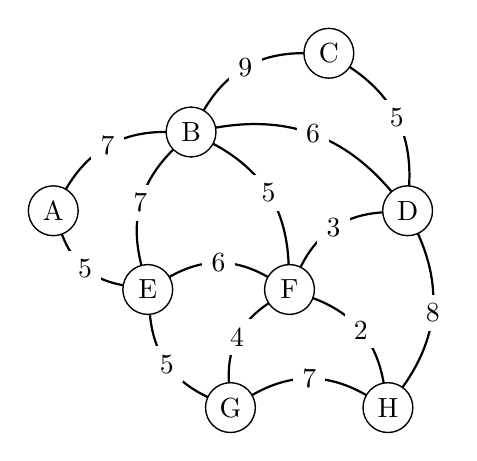
\begin{tikzpicture}

    \Vertex[x=-1,y=2]{A}
    \Vertex[x=0.75,y=3]{B}
    \Vertex[x=0.2,y=1]{E}
    \Vertex[x=2,y=1]{F}
    \Vertex[x=2.5,y=4]{C}
    \Vertex[x=3.5,y=2]{D}
    \Vertex[x=1.25,y=-0.5]{G}
    \Vertex[x=3.25,y=-0.5]{H}
    \tikzset{EdgeStyle/.append style = {bend left}}
    \Edge[label = $7$](A)(B)
    \Edge[label = $9$](B)(C)
    \Edge[label = $5$](C)(D)
    \Edge[label = $8$](D)(H)
    \Edge[label = $7$](G)(H)
    \Edge[label = $5$](G)(E)
    \Edge[label = $4$](G)(F)
    \Edge[label = $2$](F)(H)
    \Edge[label = $6$](E)(F)
    \Edge[label = $5$](E)(A)
    \Edge[label = $3$](F)(D)
    \Edge[label = $7$](E)(B)
    \Edge[label = $5$](B)(F)
    \Edge[label = $6$](B)(D)
    % \tikzset{EdgeStyle/.append style = {bend right}}
    
    \end{tikzpicture}
    \end{center}

    \textbf{Answer.}
    

    \begin{enumerate}
        \item State 1:

        \begin{center}
        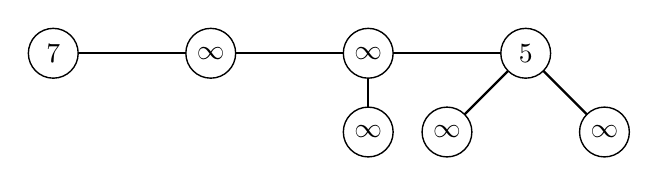
\begin{tikzpicture}
    
        \Vertex[Math,L=7,x=0,y=0]{1}
        \Vertex[Math,L=\infty,x=2,y=0]{7}
        \Vertex[Math,L=\infty,x=4,y=0]{6}
        \Vertex[Math,L=\infty,x=4,y=-1]{5}
        \Vertex[Math,L=5,x=6,y=0]{4}
        \Vertex[Math,L=\infty,x=5,y=-1]{2}
        \Vertex[Math,L=\infty,x=7,y=-1]{3}
        
        \Edge[](1)(7)
        \Edge[](7)(6)
        \Edge[](6)(5)
        \Edge[](6)(4)
        \Edge[](4)(2)
        \Edge[](4)(3)
        
        \end{tikzpicture}
        \end{center}

        \item State 2:

        \begin{center}
        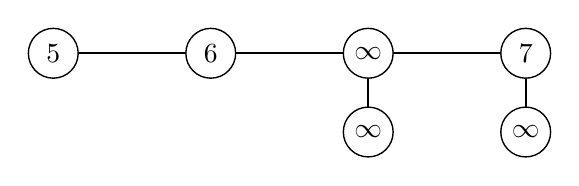
\begin{tikzpicture}
    
        \Vertex[Math,L=5,x=0,y=0]{6}
        \Vertex[Math,L=6,x=2,y=0]{5}
        \Vertex[Math,L=\infty,x=4,y=0]{2}
        \Vertex[Math,L=\infty,x=4,y=-1]{3}
        \Vertex[Math,L=7,x=6,y=0]{1}
        \Vertex[Math,L=\infty,x=6,y=-1]{7}
        
        \Edge[](6)(5)
        \Edge[](5)(2)
        \Edge[](2)(3)
        \Edge[](2)(1)
        \Edge[](1)(7)
        
        \end{tikzpicture}
        \end{center}

        \item State 3:

        \begin{center}
        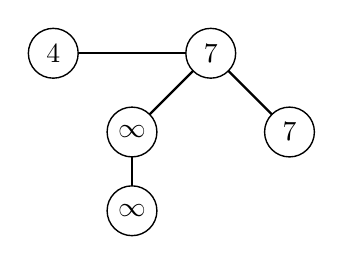
\begin{tikzpicture}
    
        \Vertex[Math,L=4,x=0,y=0]{5}
        \Vertex[Math,L=7,x=2,y=0]{1}
        \Vertex[Math,L=\infty,x=1,y=-1]{2}
        \Vertex[Math,L=\infty,x=1,y=-2]{3}
        \Vertex[Math,L=7,x=3,y=-1]{7}
        
        \Edge[](5)(1)
        \Edge[](1)(2)
        \Edge[](1)(7)
        \Edge[](2)(3)
        
        \end{tikzpicture}
        \end{center}

        \item State 4:

        \begin{center}
        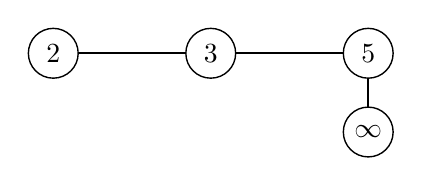
\begin{tikzpicture}
    
        \Vertex[Math,L=2,x=0,y=0]{7}
        \Vertex[Math,L=3,x=2,y=0]{3}
        \Vertex[Math,L=5,x=4,y=0]{1}
        \Vertex[Math,L=\infty,x=4,y=-1]{2}
        
        \Edge[](7)(3)
        \Edge[](3)(1)
        \Edge[](1)(2)
        
        \end{tikzpicture}
        \end{center}

        \item State 5:

        \begin{center}
        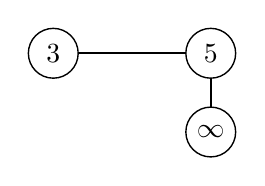
\begin{tikzpicture}
    
        \Vertex[Math,L=3,x=0,y=0]{3}
        \Vertex[Math,L=5,x=2,y=0]{1}
        \Vertex[Math,L=\infty,x=2,y=-1]{2}
        
        \Edge[](3)(1)
        \Edge[](1)(2)
        
        \end{tikzpicture}
        \end{center}

        \item State 6:

        \begin{center}
        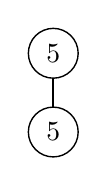
\begin{tikzpicture}
    
        \Vertex[Math,L=5,x=0,y=0]{1}
        \Vertex[Math,L=5,x=0,y=-1]{2}
        
        \Edge[](1)(2)
        
        \end{tikzpicture}
        \end{center}

        \item State 7:

        \begin{center}
        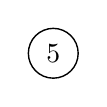
\begin{tikzpicture}
    
        \Vertex[Math,L=5,x=0,y=0]{2}
        
        \end{tikzpicture}
        \end{center}

        \item State 8:

        \begin{center}
        \begin{tikzpicture}
        
        \end{tikzpicture}
        \end{center}
    \end{enumerate}

    \item Suppose that all edge weights in a graph are integers in the range from 1 to $|V|$. How fast can you make Prim-Jarnik algorithm run? What if the edge weights are integers in the range from 1 to $W$ for some constant $W$? Justify your answer in at most two paragraphs.

    \textbf{Answer.}

     If the edge weights are in some range then we can create an array with size of $W$ and add edges to the corresponding weights. Therefore, we will get sorted edges by their weight. We can replace the $|V|\log{|V|}$ and $|E|\log{|V|}$ loops from \texttt{EXTRACT-MIN} and \texttt{DECREASE-KEY} operations in Prim's algorithm with the created weight array. This will change the original time complexity of $O(\log{|V|}(|V| + |E|))$ to $O(W(|V| + |E|))$.
     
\end{enumerate}

\begin{thebibliography}{9}
\bibitem{Cormen}
  T. H. Cormen, C. E. Leiserson, R. L. Rivest and C. Stein.
  \textit{Introduction to Algorithms, Fourth Edition.}
  The MIT Press
  2022.
\end{thebibliography}

\end{document}
